\documentclass{article}
\def\matH{H}
\def\matg{G}
\usepackage{tikz}
\usetikzlibrary{matrix,fit}
\pgfdeclarelayer{bg}
\pgfsetlayers{bg,main}
\begin{document}
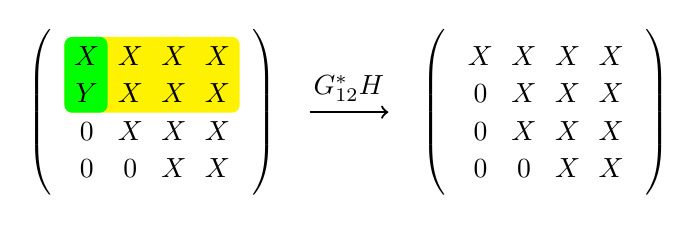
\begin{tikzpicture}
  \node
[matrix of math nodes,left delimiter=(,right delimiter=)] (m)  at (0,0)
{
  X&X&X&X\\
  Y&X&X&X\\
  0&X&X&X\\
  0&0&X&X\\
};

\node
[matrix of math nodes,left delimiter=(,right delimiter=)] (r)  at (5,0)
{
  X&X&X&X\\
  0&X&X&X\\
  0&X&X&X\\
  0&0&X&X\\
};

\draw[->,thick] (2,0) -- node[above] {$\matg_{12}^*\matH$} (3,0);

\begin{pgfonlayer}{bg}
  \node[fit={(m-1-1.north west) (m-2-4.south east)},fill=yellow,inner sep=0,rounded corners=1mm]{};
  \node[fit={(m-1-1.north west) (m-2-1.south east)},fill=green,inner sep=0,rounded corners=1mm]{};
\end{pgfonlayer}

;
\end{tikzpicture}


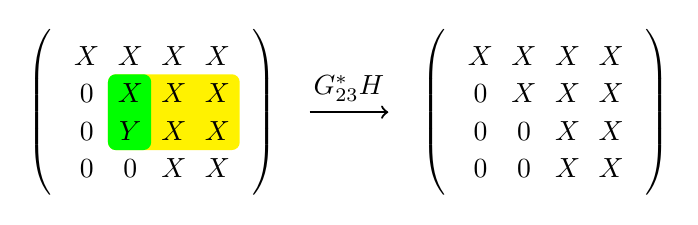
\begin{tikzpicture}
  \matrix
[matrix of math nodes,left delimiter=(,right delimiter=)] (m)
{
  X&X&X&X\\
  0&X&X&X\\
  0&Y&X&X\\
  0&0&X&X\\
};

\node
[matrix of math nodes,left delimiter=(,right delimiter=)] (r)  at (5,0)
{
  X&X&X&X\\
  0&X&X&X\\
  0&0&X&X\\
  0&0&X&X\\
};

\draw[->,thick] (2,0) -- node[above] {$\matg_{23}^*\matH$} (3,0);

\begin{pgfonlayer}{bg}
  \node[fit={(m-2-2.north west) (m-3-4.south east)},fill=yellow,inner sep=0,rounded corners=1mm]{};
  \node[fit={(m-2-2.north west) (m-3-2.south east)},fill=green,inner sep=0,rounded corners=1mm]{};
\end{pgfonlayer}
;
\end{tikzpicture}

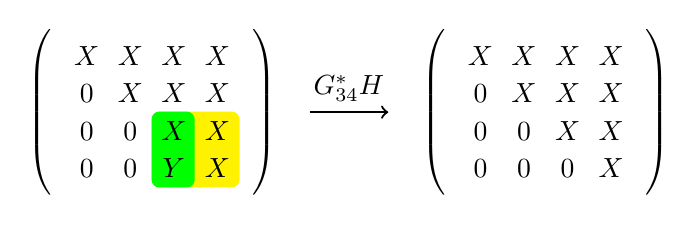
\begin{tikzpicture}
  \matrix
[matrix of math nodes,left delimiter=(,right delimiter=)] (m)
{
  X&X&X&X\\
  0&X&X&X\\
  0&0&X&X\\
  0&0&Y&X\\
};

\node
[matrix of math nodes,left delimiter=(,right delimiter=)] (r)  at (5,0)
{
  X&X&X&X\\
  0&X&X&X\\
  0&0&X&X\\
  0&0&0&X\\
};

\draw[->,thick] (2,0) -- node[above] {$\matg_{34}^*\matH$} (3,0);

\begin{pgfonlayer}{bg}
  \node[fit={(m-3-3.north west) (m-4-4.south east)},fill=yellow,inner sep=0,rounded corners=1mm]{};
  \node[fit={(m-3-3.north west) (m-4-3.south east)},fill=green,inner sep=0,rounded corners=1mm]{};
\end{pgfonlayer}
;
\end{tikzpicture}

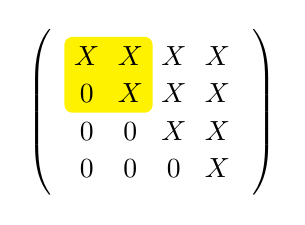
\begin{tikzpicture}
  \matrix
[matrix of math nodes,left delimiter=(,right delimiter=)] (m)
{
  X&X&X&X\\
  0&X&X&X\\
  0&0&X&X\\
  0&0&0&X\\
};
\begin{pgfonlayer}{bg}
  \node[fit={(m-1-1.north west) (m-2-2.south east)},fill=yellow,inner sep=0,rounded corners=1mm]{};
\end{pgfonlayer}
;
\end{tikzpicture}
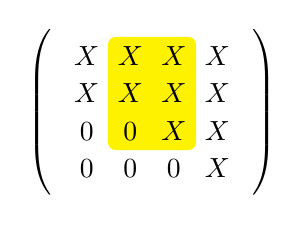
\begin{tikzpicture}
  \matrix
[matrix of math nodes,left delimiter=(,right delimiter=)] (m)
{
  X&X&X&X\\
  X&X&X&X\\
  0&0&X&X\\
  0&0&0&X\\
};
\begin{pgfonlayer}{bg}
  \node[fit={(m-1-2.north west) (m-3-3.south east)},fill=yellow,inner sep=0,rounded corners=1mm]{};
\end{pgfonlayer}
;
\end{tikzpicture}
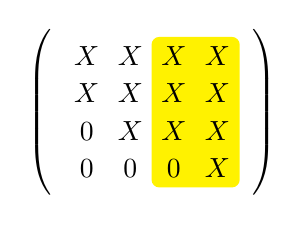
\begin{tikzpicture}
  \matrix
[matrix of math nodes,left delimiter=(,right delimiter=)] (m)
{
  X&X&X&X\\
  X&X&X&X\\
  0&X&X&X\\
  0&0&0&X\\
};
\begin{pgfonlayer}{bg}
  \node[fit={(m-1-3.north west) (m-4-4.south east)},fill=yellow,inner sep=0,rounded corners=1mm]{};
\end{pgfonlayer}
;
\end{tikzpicture}
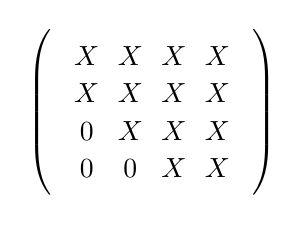
\begin{tikzpicture}
  \matrix
[matrix of math nodes,left delimiter=(,right delimiter=)] (m)
{
  X&X&X&X\\
  X&X&X&X\\
  0&X&X&X\\
  0&0&X&X\\
};
;
\end{tikzpicture}

\end{document}
